\subsection{Standard Model \ttbar+Z}
\label{sec:Bkg:ttV}

$\ttbar$ produced in conjunction with a Z boson consist of about 1 percent of the background in the SR.  Although the background is essentially negligible we do estimate the amount of $\ttbar+\Zboson$ using a $\ttbar+\gamma$ CR. Designing a CR to estimate the $\ttbar+Z$ background by using the charged leptonic $Z$ boson decays would be favorable. However, such CR is difficult to design due to low statistics and the small branching fraction to leptons. In particular a 2-lepton CR suffers from a large contamination of $\ttbar$ and $Z$ + jets processes. For this reason, another data driven approach is followed by building a one-lepton CR for $\ttbar\gamma$ which is a similar process. A zero-lepton region was considered as a validation region but it was found to have a too low $\ttbar\gamma$ contribution, with $\gamma$+jets being the main contaminant.\\
The CR is designed to minimize the differences between the two processes and keep the theoretical uncertainties from the extrapolation of the $\gamma$ to the \Zboson\ low. \\

The $\ttbar+\gamma$ CR requires exactly one photon with a FixedCutTight isolation WP, exactly one signal lepton (electron or muon as defined in Section~\ref{sec:Selection}) and at least four jets of which at least two are required to be b-tagged. To collect these events the lepton triggers described in Table~\ref{tb:lepTriggers} are used. \\
Moreover, due to the difference in mass between the \Zboson\ and the $\gamma$, to mimic the $Z \rightarrow \nu\nu$ decay, the highest \pT\ photon is required to have $\pt>150\gev$. \\ %A k-factor equal to 1.47~\cite{ATLAS:xsecNLOttV} is applied to $\ttbar\gamma$. 
Unlike the CRTops, CRW, and CRST one-lepton control regions the lepton is not treated as a jet. Instead, the photon is used to model the \met\ since the \met\ from $\ttbar+Z$ in the SR originates mostly from the neutrino decay of the \Zboson. \\
The details of the selection for the one-lepton CR are summarized in Table~\ref{tb:ttG_1lepSel}.\\


\begin{table}[htpb]
  \caption{Selection for the $\ttbar+\gamma$ 1 lepton CR. The same triggers as described in Table~\ref{tb:lepTriggers} are used and the same signal lepton requirements are mad as in Tables~\ref{tb:electronsSignal} and~\ref{tb:muonsSignal}}
  \begin{center}
    \begin{tabular}{c|c}
      \hline \hline
      Selection                 & Requirement     \\
      \hline \hline
      Event selection & Event cleaning \\
      \hline
      % Trigger (Data 2015) &\texttt{HLT\_g120\_loose}  \\ 
      % \hline
      % Trigger (Data 2016) & \texttt{HLT\_g140\_loose}  \\ 
      %\hline
      Leptons & exactly 1 \\
      Lepton \pt & 28 GeV \\
      \hline
      Photons & exactly 1\\
      \hline
      jet multiplicity & $ \ge 4 $ \\
      \hline
      Jet \pT\ & (80,80,40,40) GeV \\
      \hline
      b-jet multiplicity & $\ge 2$ \\
      \hline
      $\gamma$ \pT\ & $> 150$ GeV \\
      \hline\hline
    \end{tabular}
  \end{center}
  \label{tb:ttG_1lepSel}
\end{table}


Table~\ref{tb:ttVCR_2bj} shows the background composition for the $\ttbar\gamma$ CR. A normalisation factor is derived as the ratio between data and MC correcting for the contamination for non-$t\bar{t}\gamma$ backgrounds.


\begin{table}[htpb]
  \caption{Background composition of $t\bar{t}\gamma$ CR.}
  \begin{center}
\begin{tabular}{c|c}
\hline\hline
\multicolumn{2}{c}{\bf CRTTGamma (87\% purity)} \\ \hline 
ttGamma & 112.20 $\pm$ 1.49 \\
VGamma & 6.41 $\pm$ 0.70 \\
Z & 0.73 $\pm$ 0.21 \\
dibosons & 0.00 $\pm$ 0.00 \\
ttbar & 4.57 $\pm$ 1.23 \\
singleTop & 2.01 $\pm$ 0.81 \\
ttV & 2.42 $\pm$ 0.28 \\
W & 0.04 $\pm$ 0.02 \\
\hline
Total MC & 128.38 $\pm$ 2.23 \\
Data & 160.00 $\pm$ 12.65 \\
 \hline
SF & 1.28 $\pm$ 0.12 \\
\hline\hline
\end{tabular}

    
  \end{center}
  \label{tb:ttVCR_2bj}
\end{table}

Data/MC comparisons of several distributions are shown in the following figures after applying the full selection in Table~\ref{tb:ttG_1lepSel}.


\begin{figure}[htbp]
\begin{center}
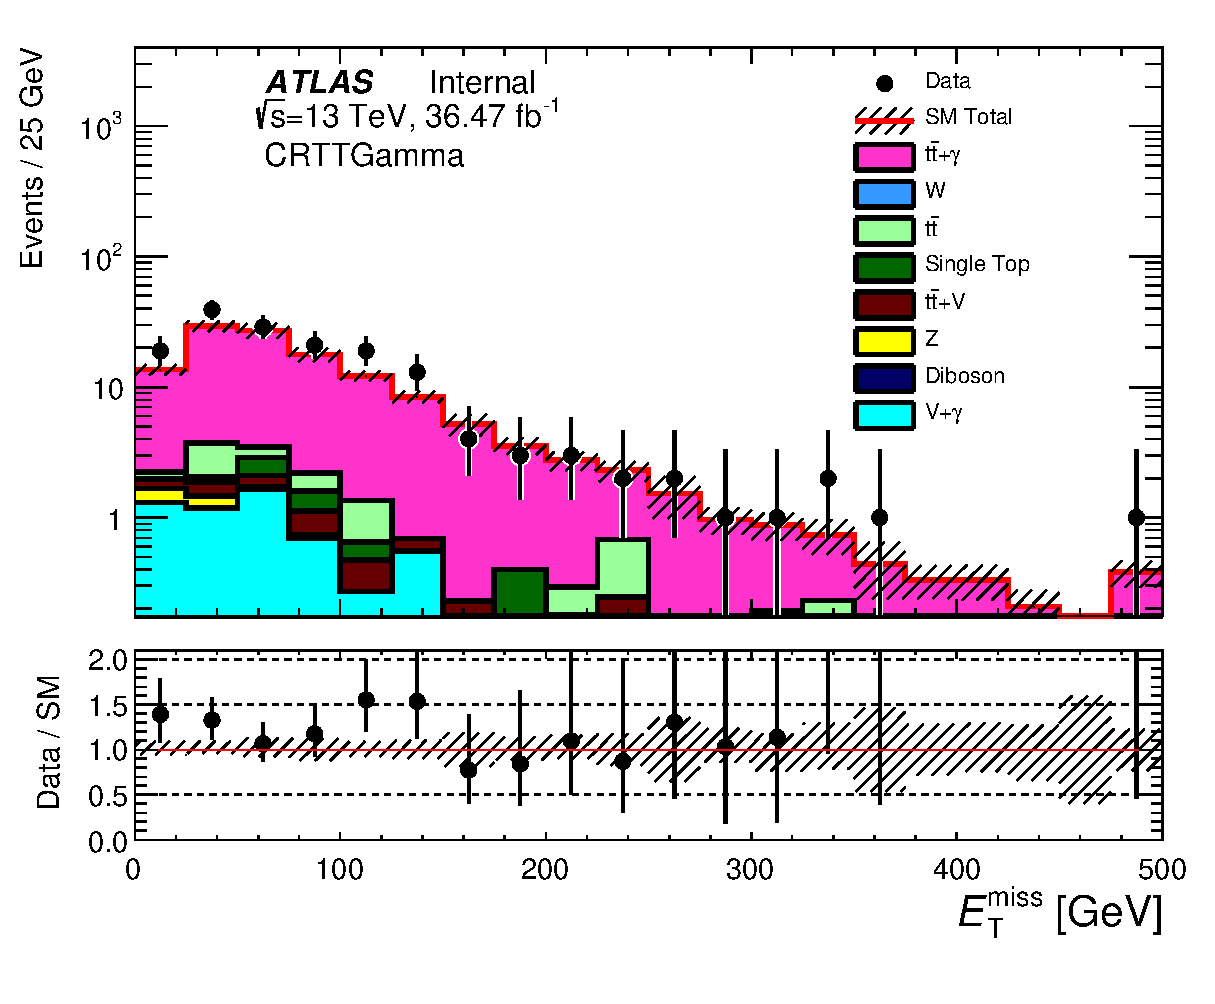
\includegraphics[width=0.49\textwidth]{figures/ttGamma/Met_CRTTGamma_withRatio_log.eps}
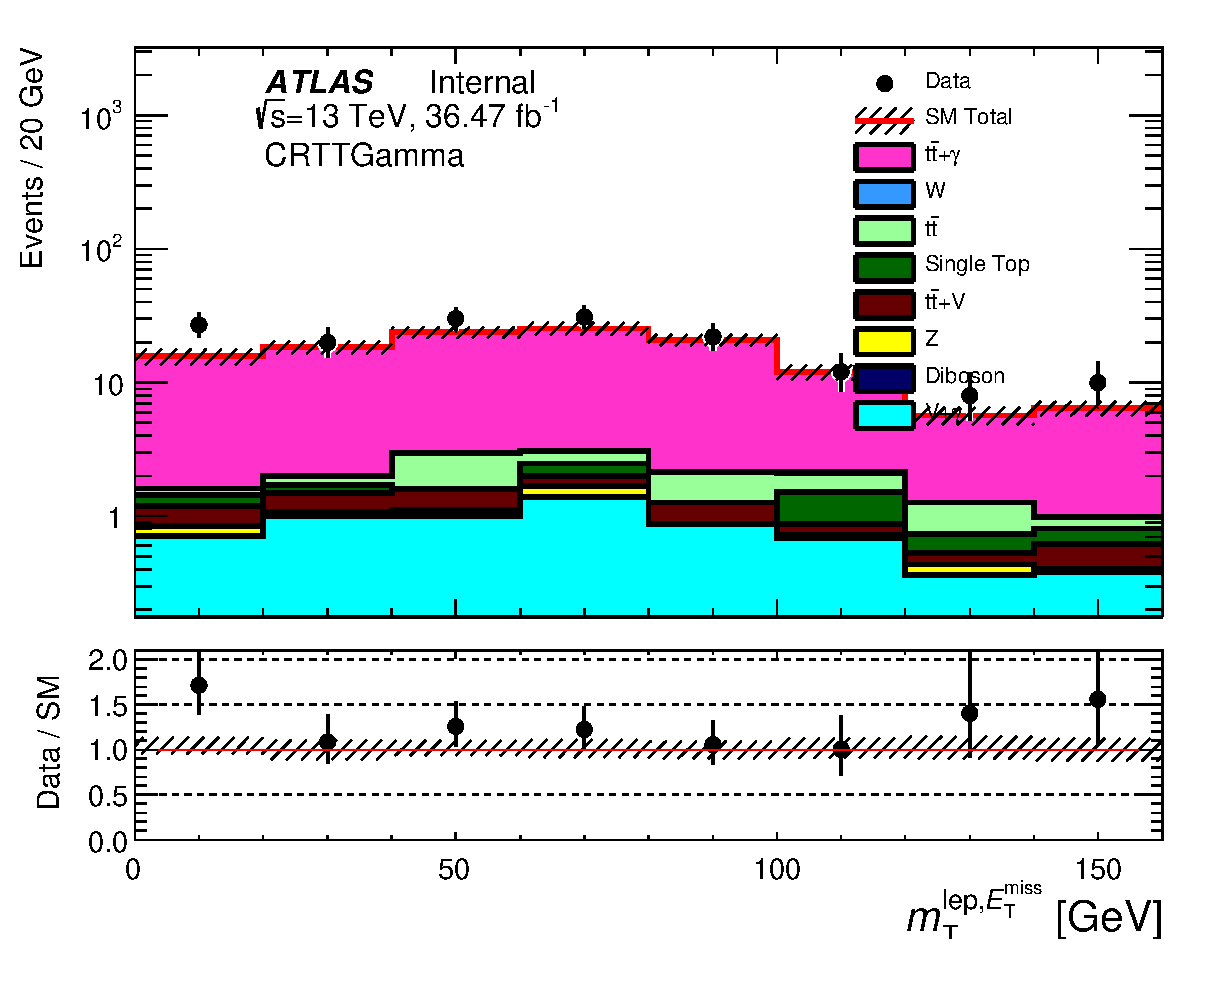
\includegraphics[width=0.49\textwidth]{figures/ttGamma/MtMetLep_CRTTGamma_withRatio_log.eps}
\caption{\label{fig:ttVFakeLepCheck} Prefit distributions of the \met\ and \mtlepmet\ for fake lepton checks. Agreement at low \mtlepmet\ is reasonable indicating no significant contributions from fake leptons. The ratio between data and MC is given in the bottom panel. The hashed area in both the top and lower panel represents the uncertainty due to MC statistics.}
\end{center}
\end{figure}

\begin{figure}[htbp]
\begin{center}
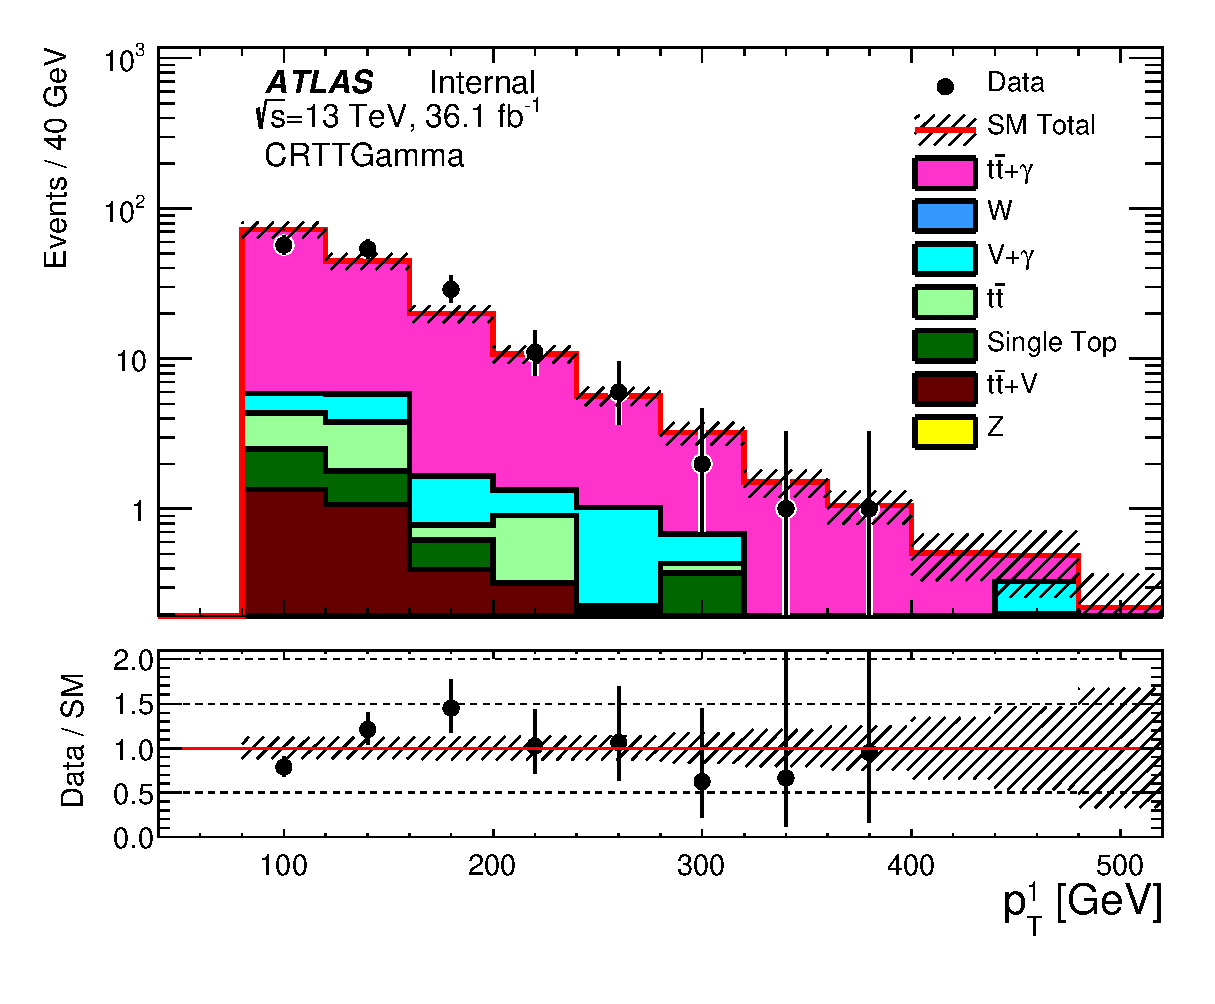
\includegraphics[width=0.49\textwidth]{figures/ttGamma/postfit/JetPt_1__CRTTGamma_log.eps}
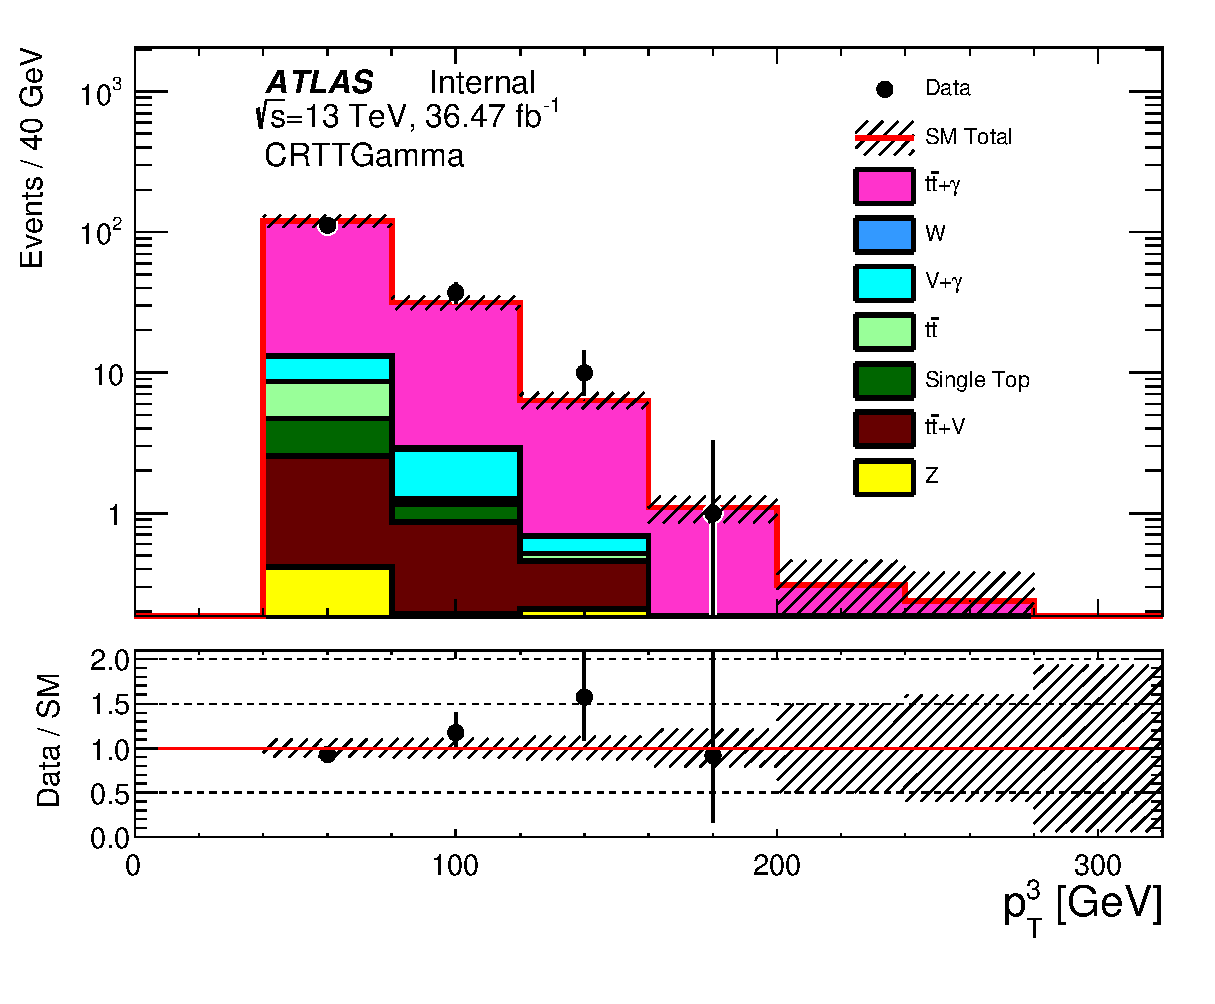
\includegraphics[width=0.49\textwidth]{figures/ttGamma/postfit/JetPt_3__CRTTGamma_log.eps}
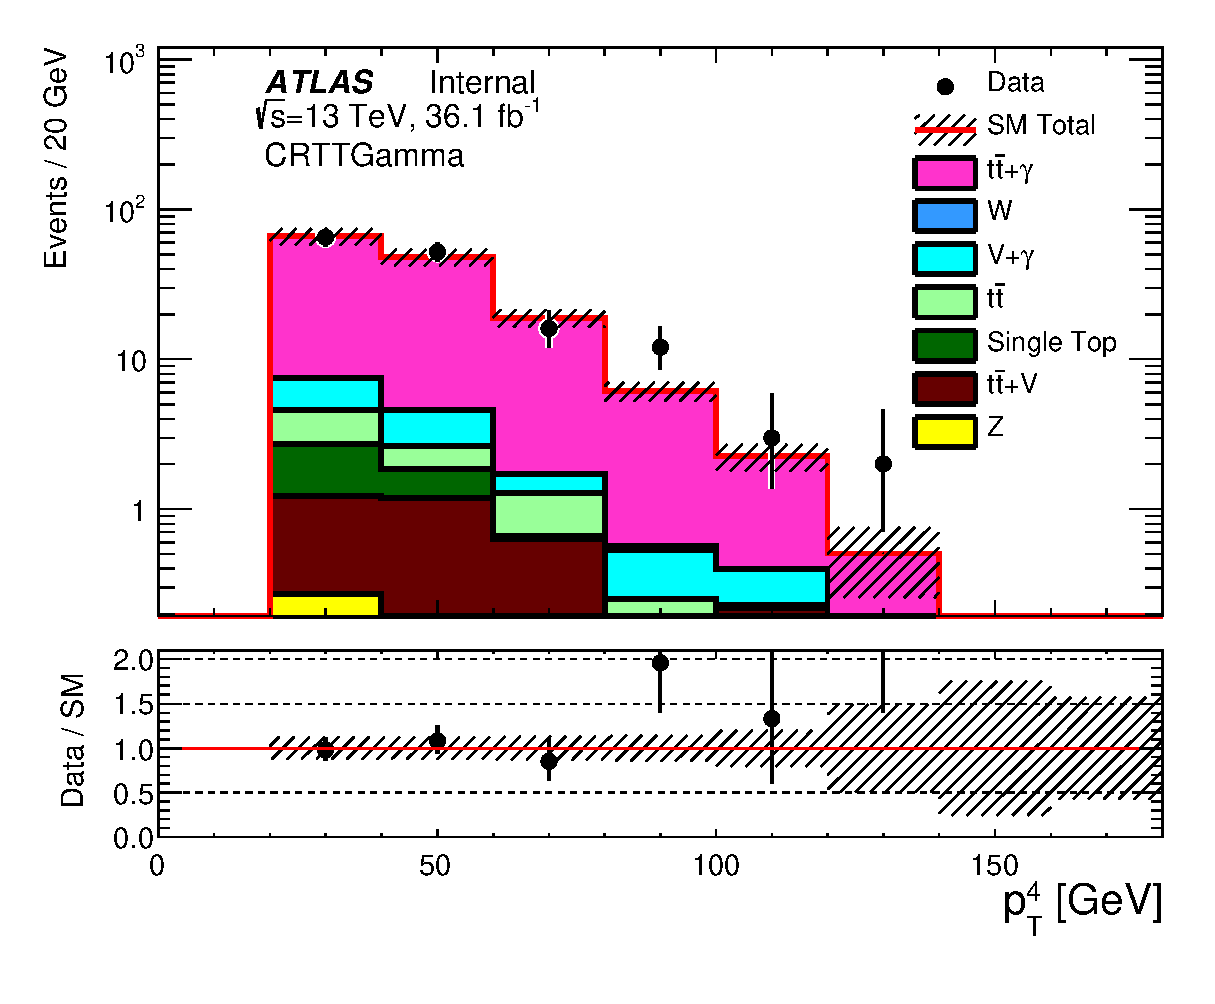
\includegraphics[width=0.49\textwidth]{figures/ttGamma/postfit/JetPt_4__CRTTGamma_log.eps}
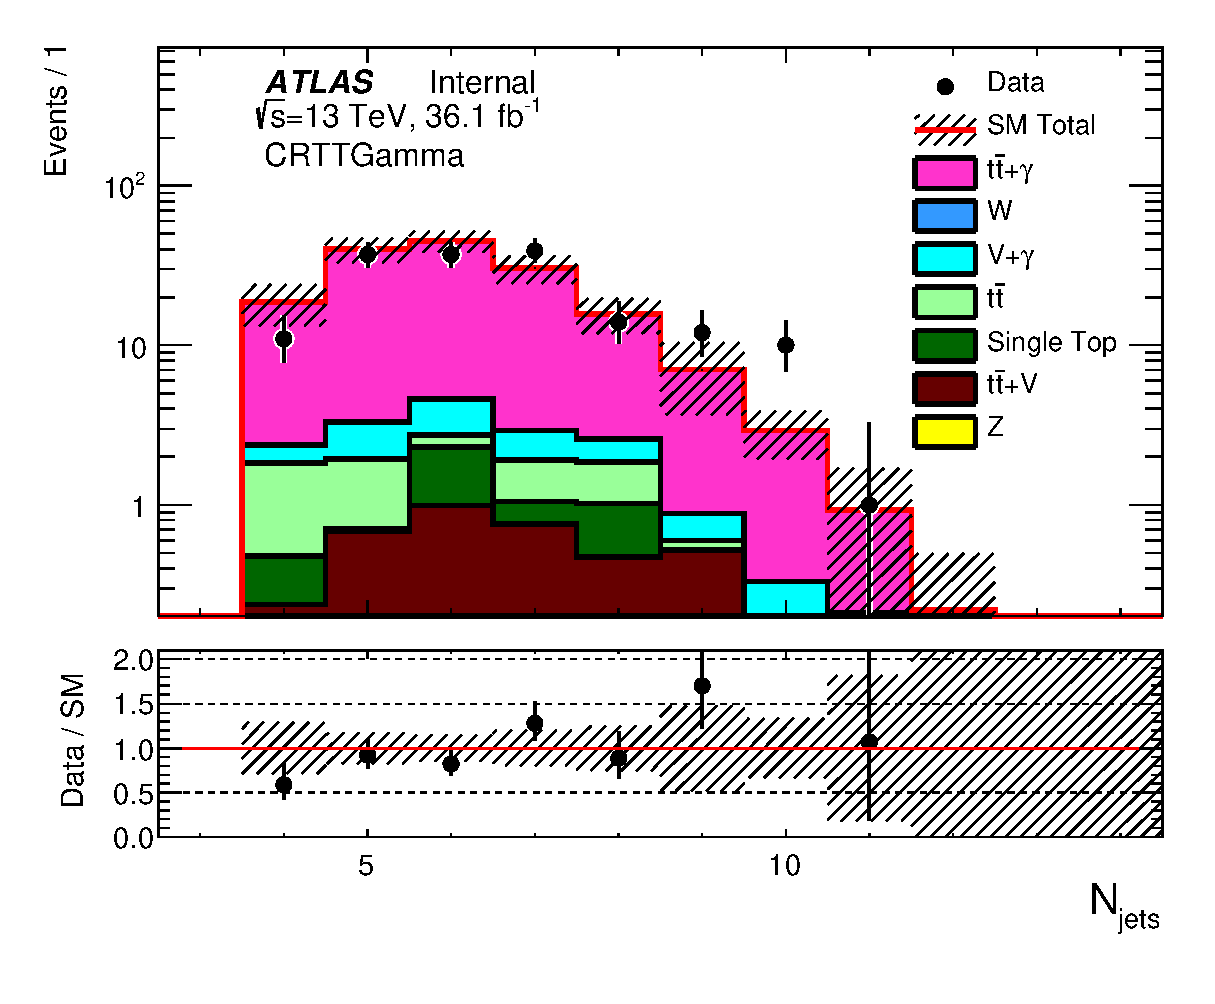
\includegraphics[width=0.49\textwidth]{figures/ttGamma/postfit/NJets_CRTTGamma_log.eps}
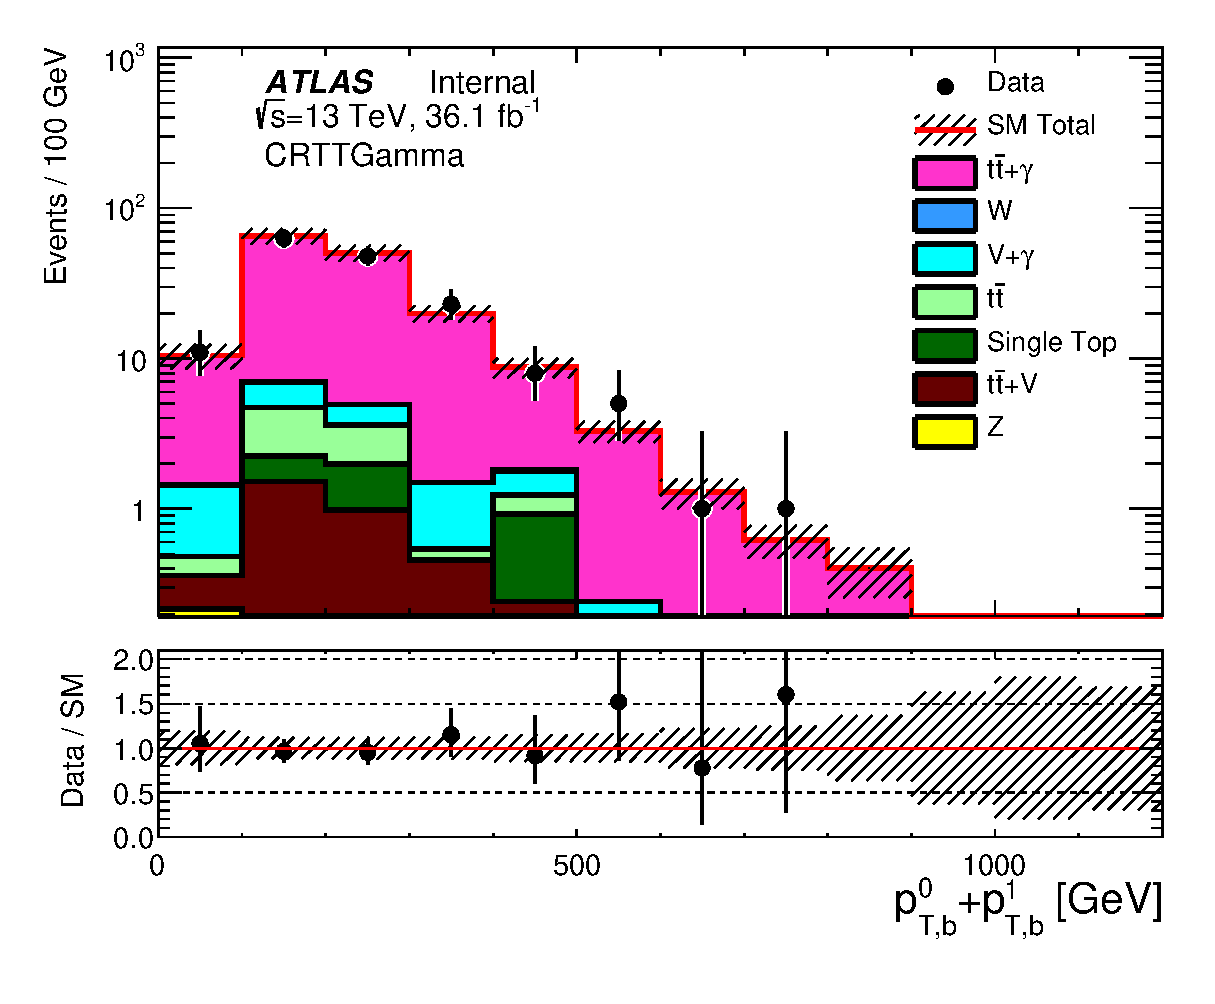
\includegraphics[width=0.49\textwidth]{figures/ttGamma/postfit/JetPt_JetLeadTagIndex_JetPt_JetSubleadTagIndex__CRTTGamma_log.eps}
\caption{\label{fig:ttVJetPts} Postfit distributions of the \pT\ of the
  leading and subleading jets for the 2 b-jets selection. The ratio between data and MC is given in the bottom panel. The hashed area in both the top and lower panel represents the uncertainty due to MC statistics.}
\end{center}
\end{figure}

\begin{figure}[htbp]
\begin{center}
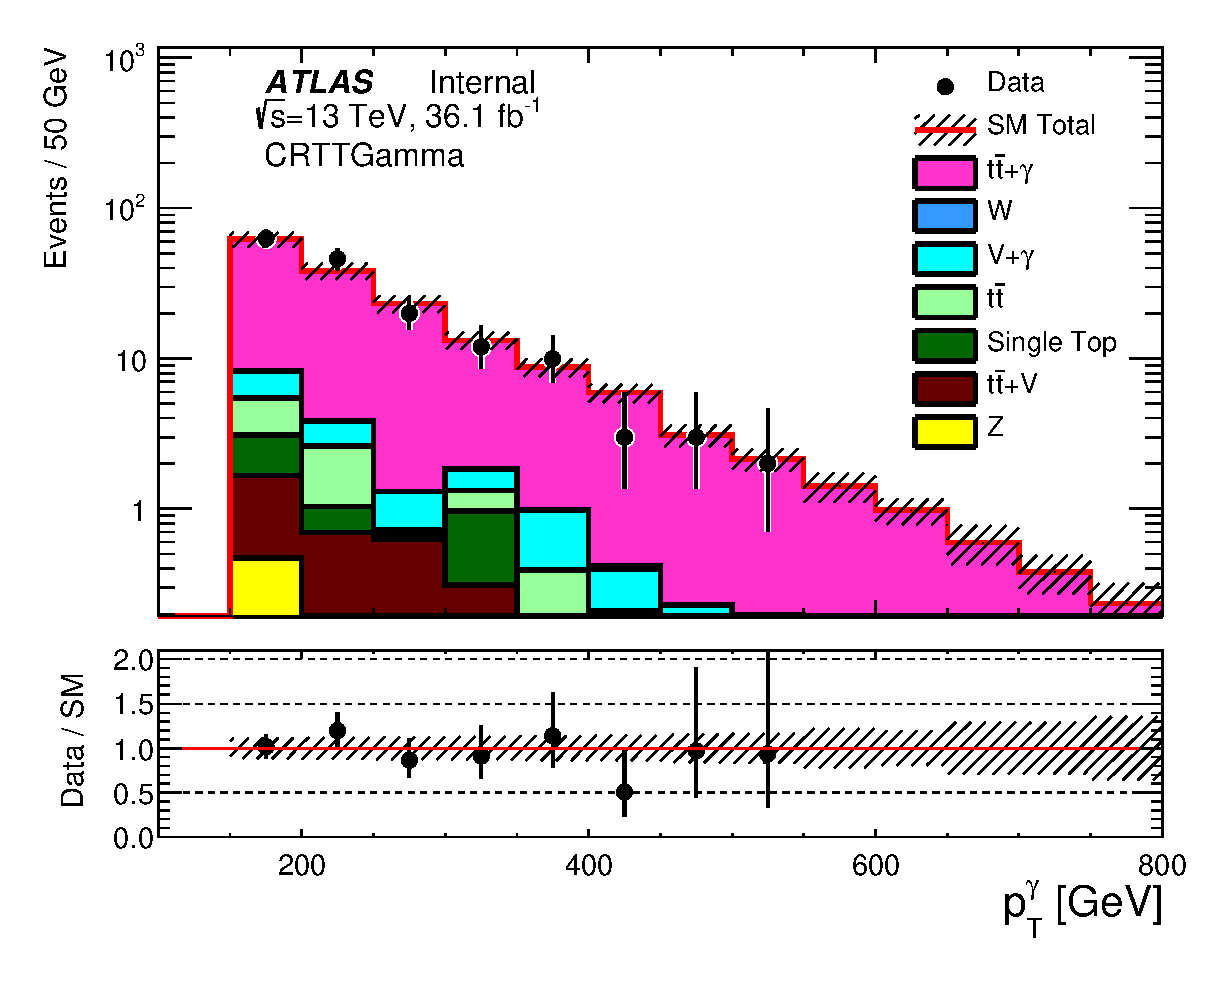
\includegraphics[width=0.49\textwidth]{figures/ttGamma/postfit/SigPhotonPt_0__CRTTGamma_log.eps}
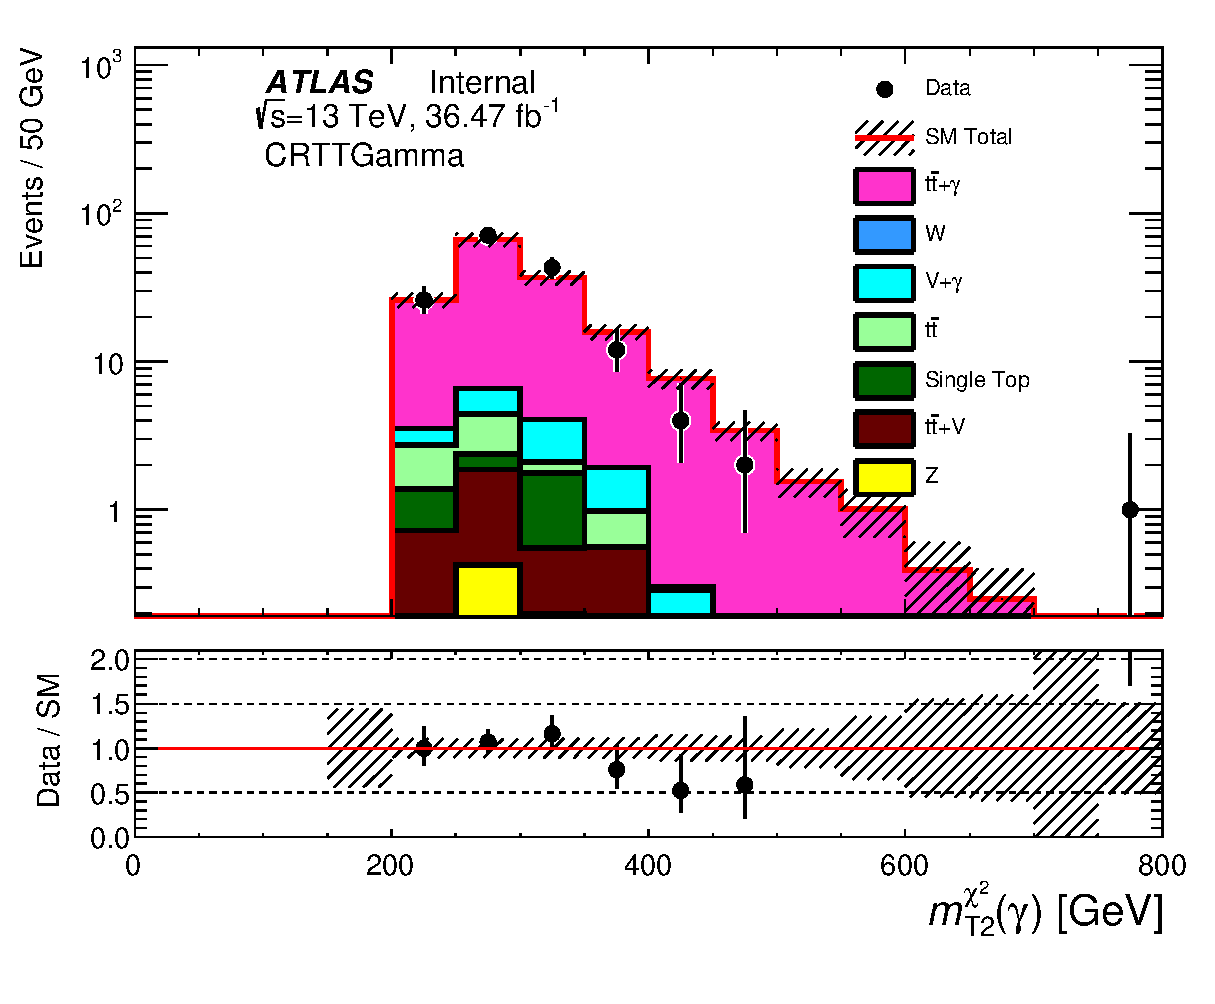
\includegraphics[width=0.49\textwidth]{figures/ttGamma/postfit/MT2Chi2Photon_CRTTGamma_log.eps}
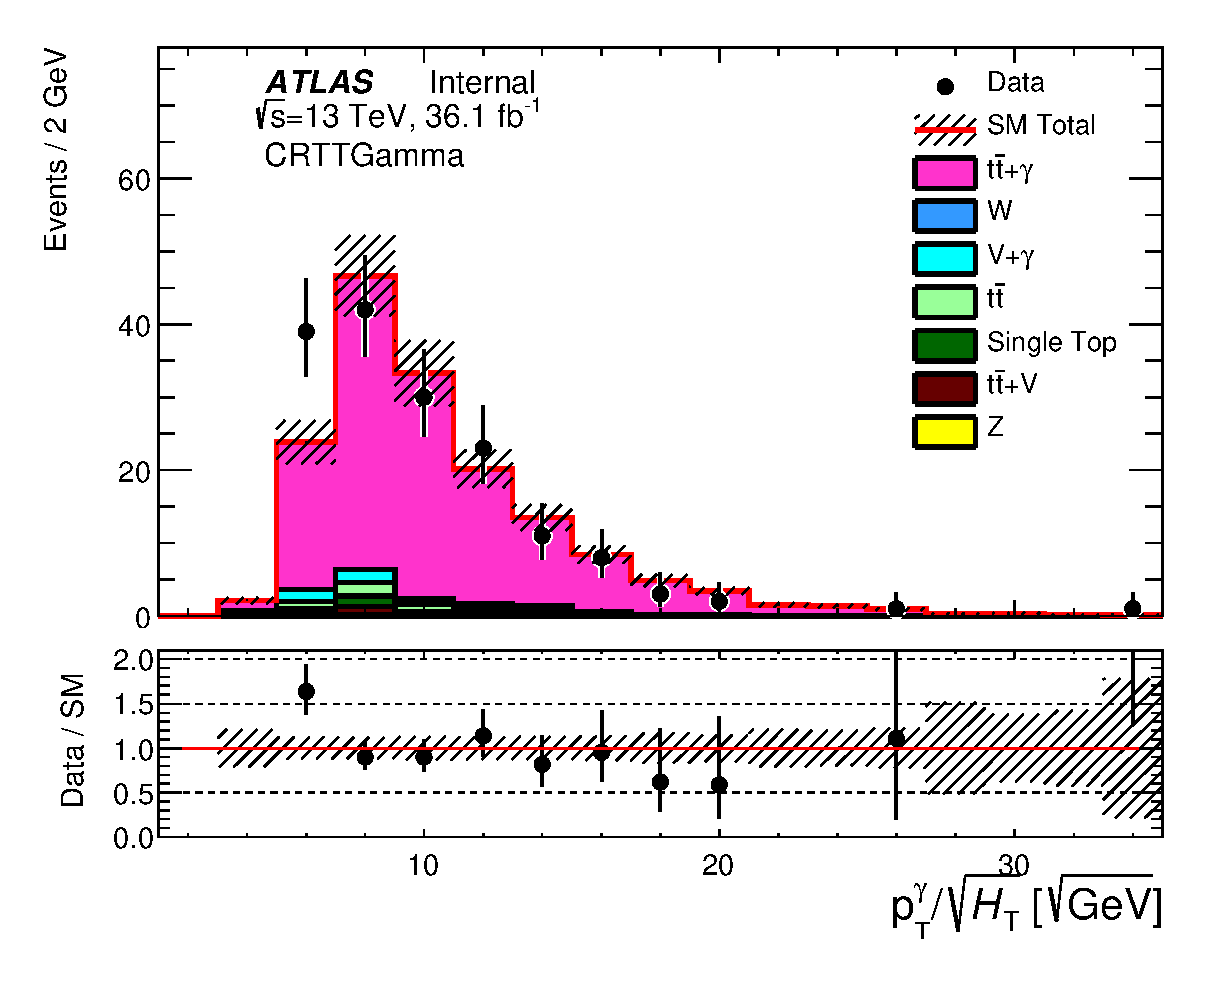
\includegraphics[width=0.49\textwidth]{figures/ttGamma/postfit/SigPhotonPt_0_sqrtHt_CRTTGamma.eps}
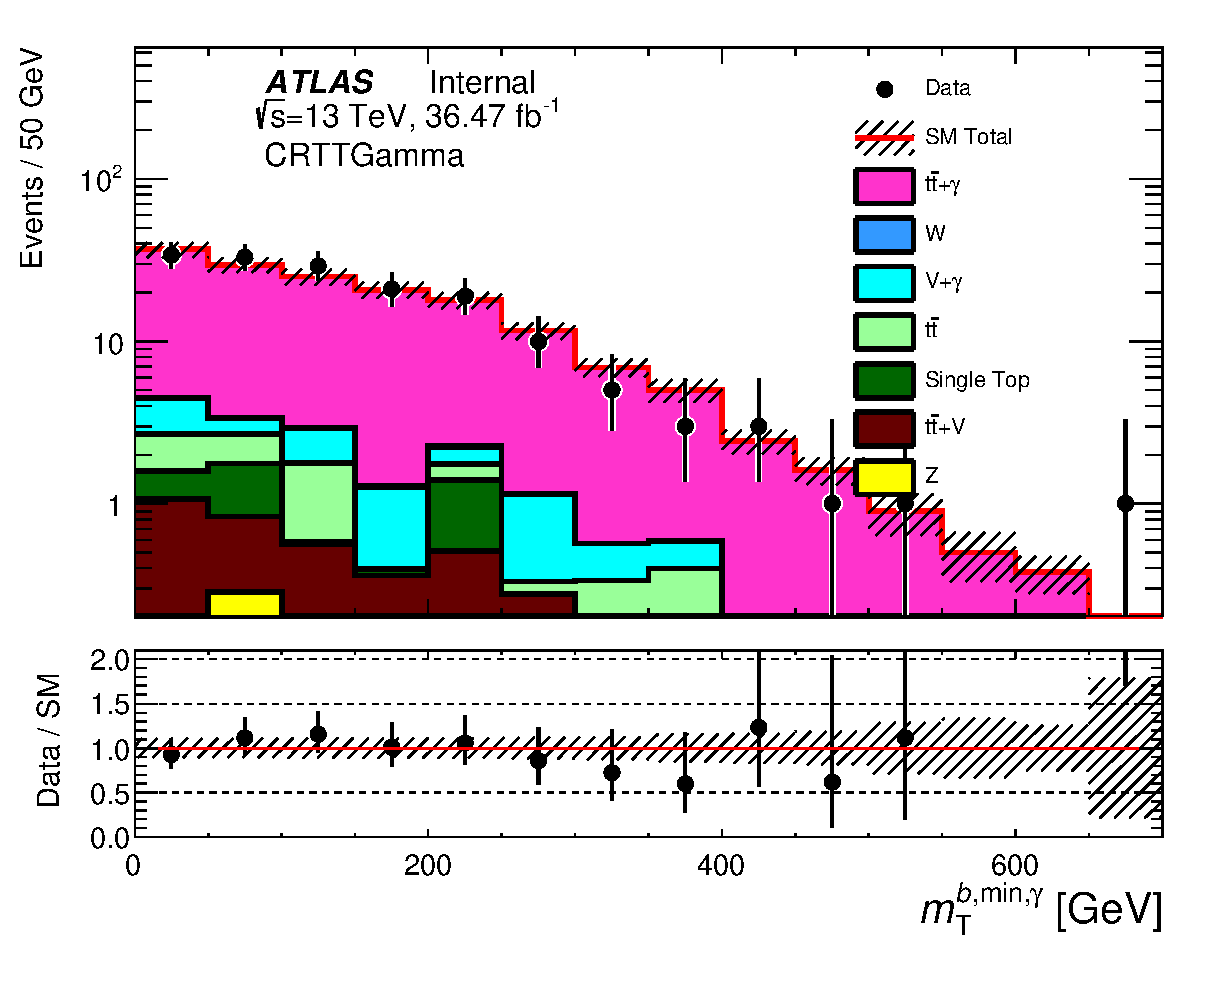
\includegraphics[width=0.49\textwidth]{figures/ttGamma/postfit/MtBMinPhoton_CRTTGamma_log.eps}
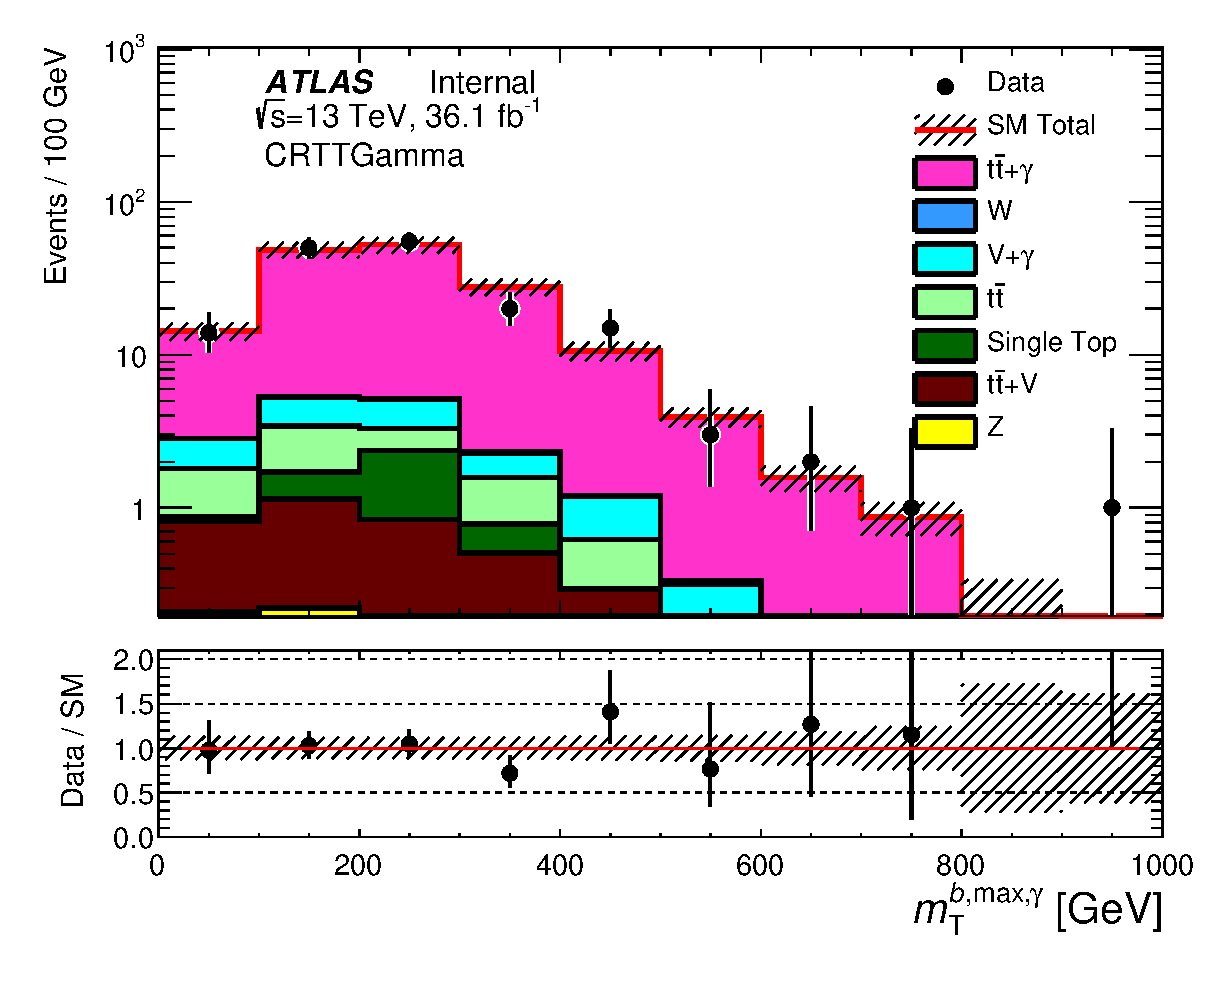
\includegraphics[width=0.49\textwidth]{figures/ttGamma/postfit/MtBMaxPhoton_CRTTGamma_log.eps}
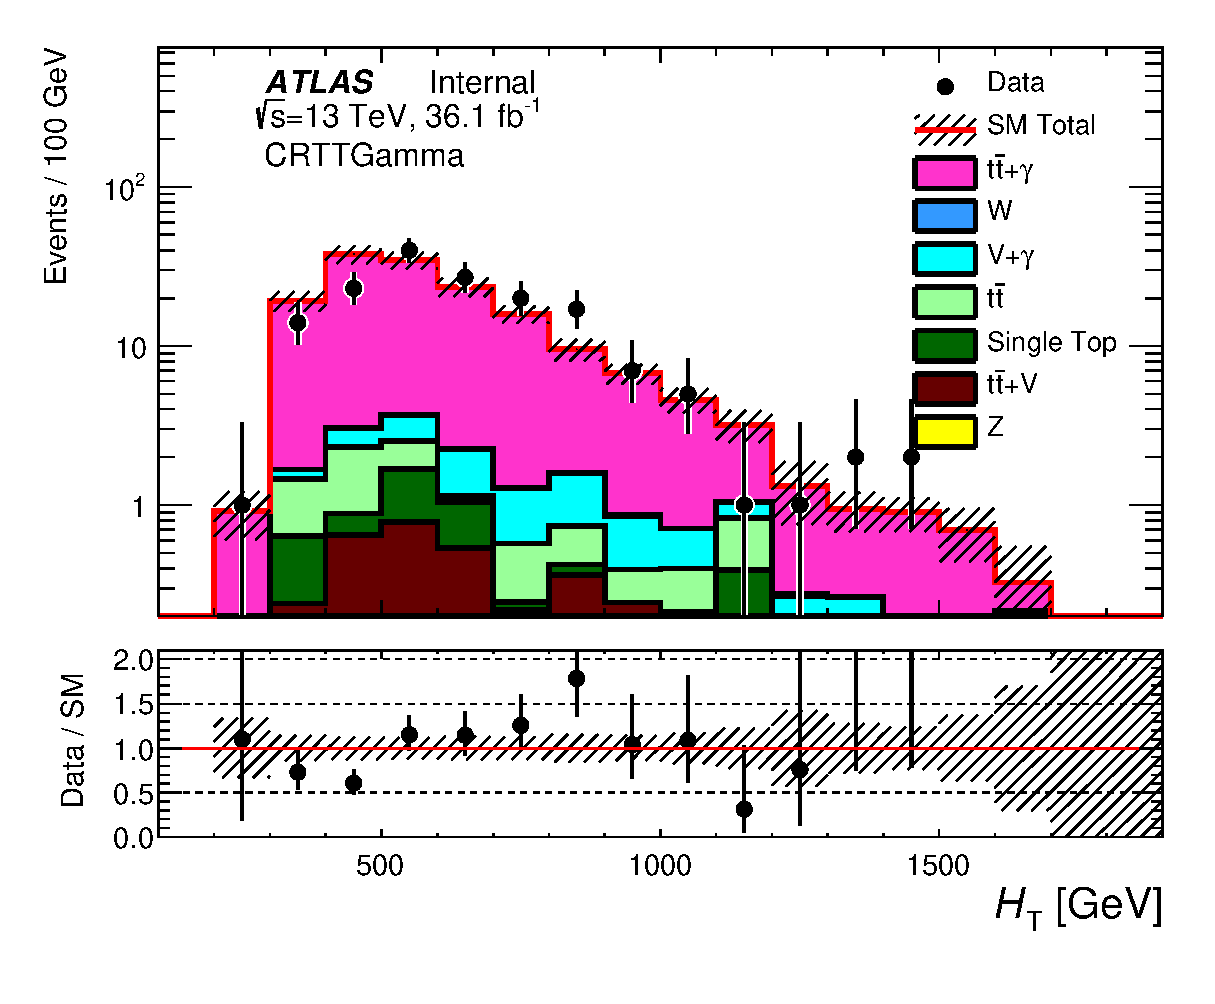
\includegraphics[width=0.49\textwidth]{figures/ttGamma/postfit/Ht_CRTTGamma_log.eps}
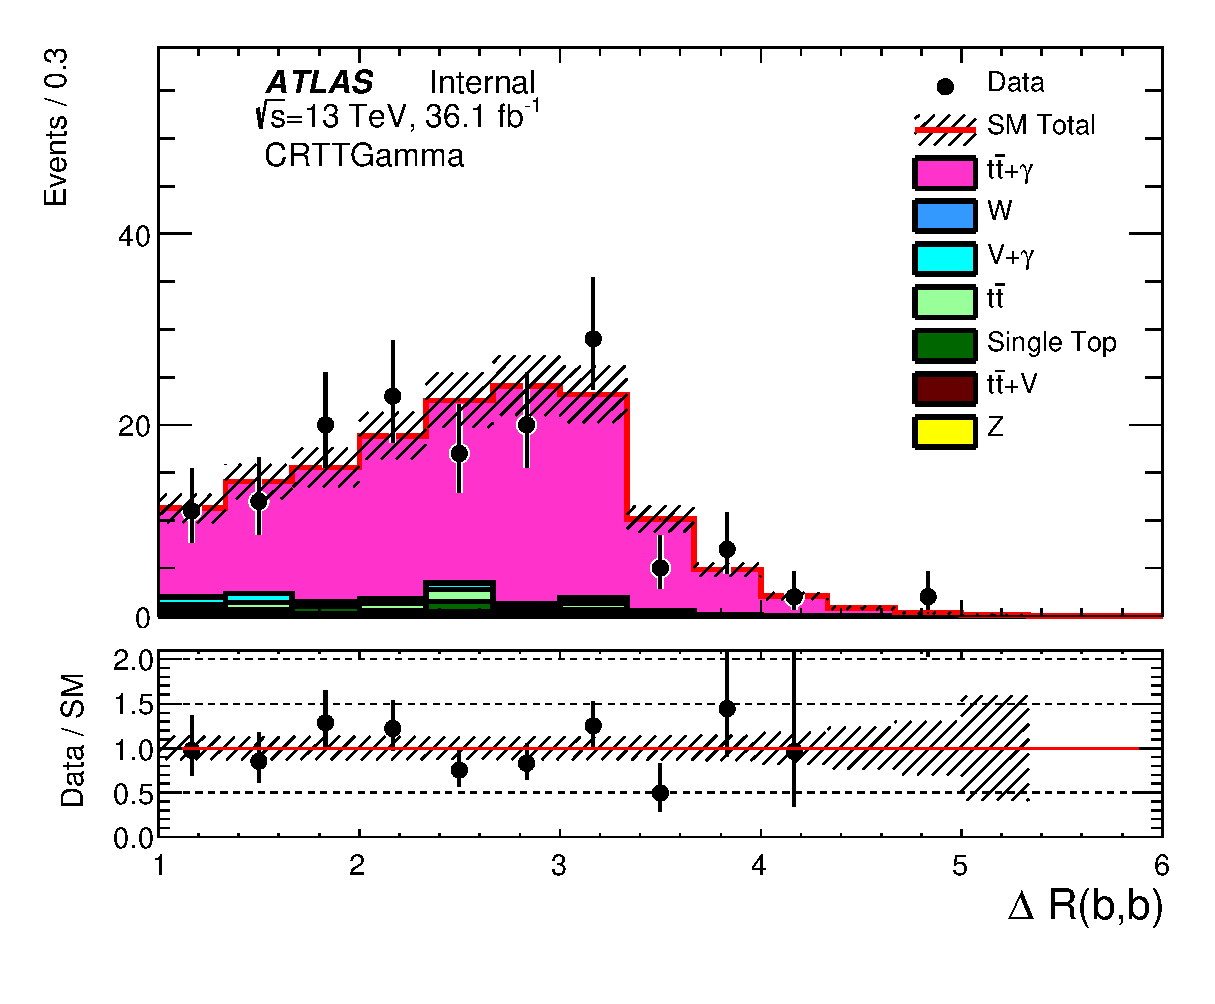
\includegraphics[width=0.49\textwidth]{figures/ttGamma/postfit/DRBB_CRTTGamma.eps}
\caption{\label{fig:ttV} Postfit distributions of the \pT\ of the
  leading and subleading jets for the 2 b-jets selection. The ratio between data and MC is given in the bottom panel. The hashed area in both the top and lower panel represents the uncertainty due to MC statistics.}
\end{center}
\end{figure}

\begin{figure}[htbp]
\begin{center}
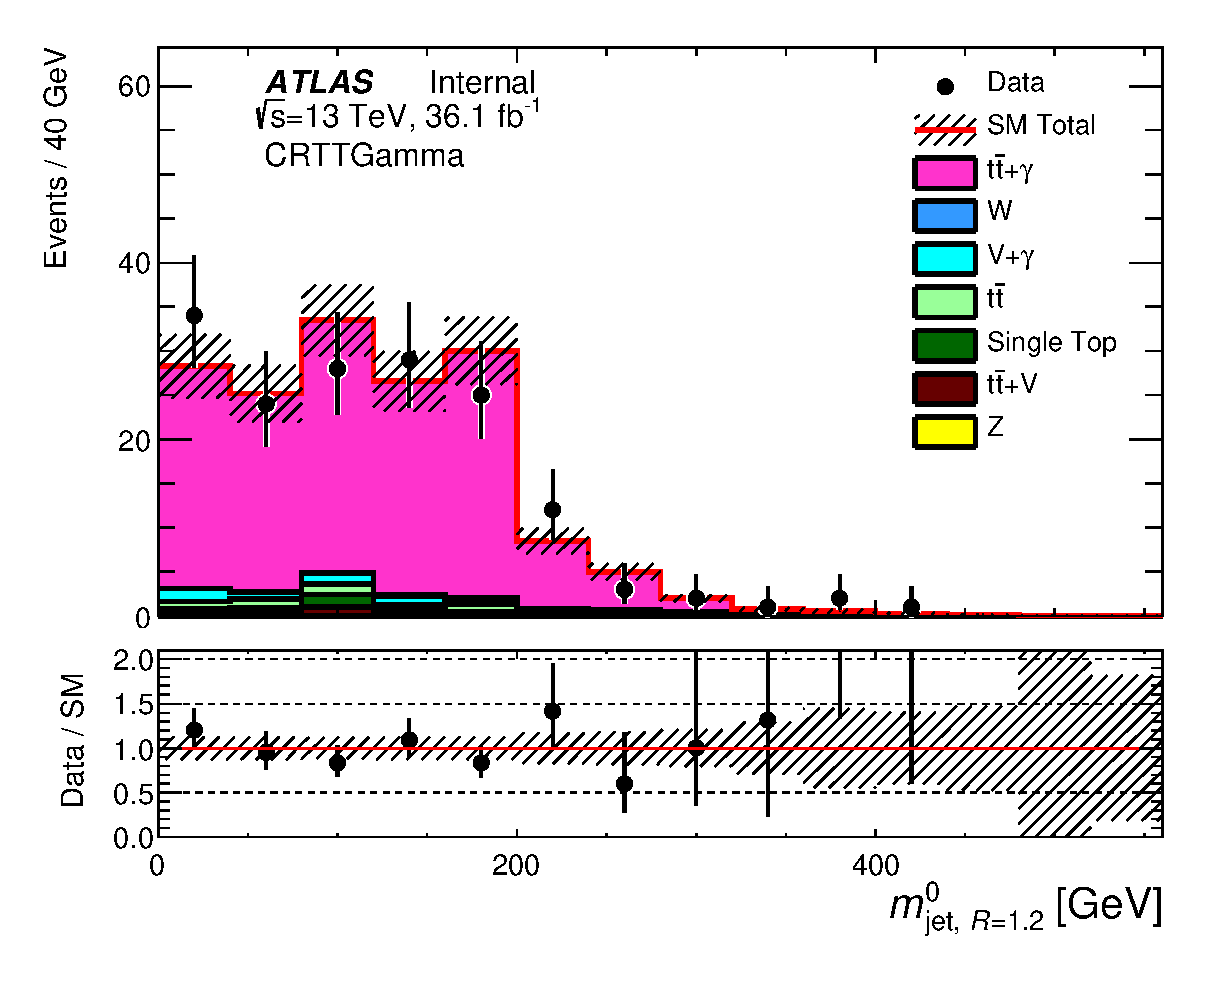
\includegraphics[width=0.49\textwidth]{figures/ttGamma/postfit/AntiKt12M_0__CRTTGamma.eps}
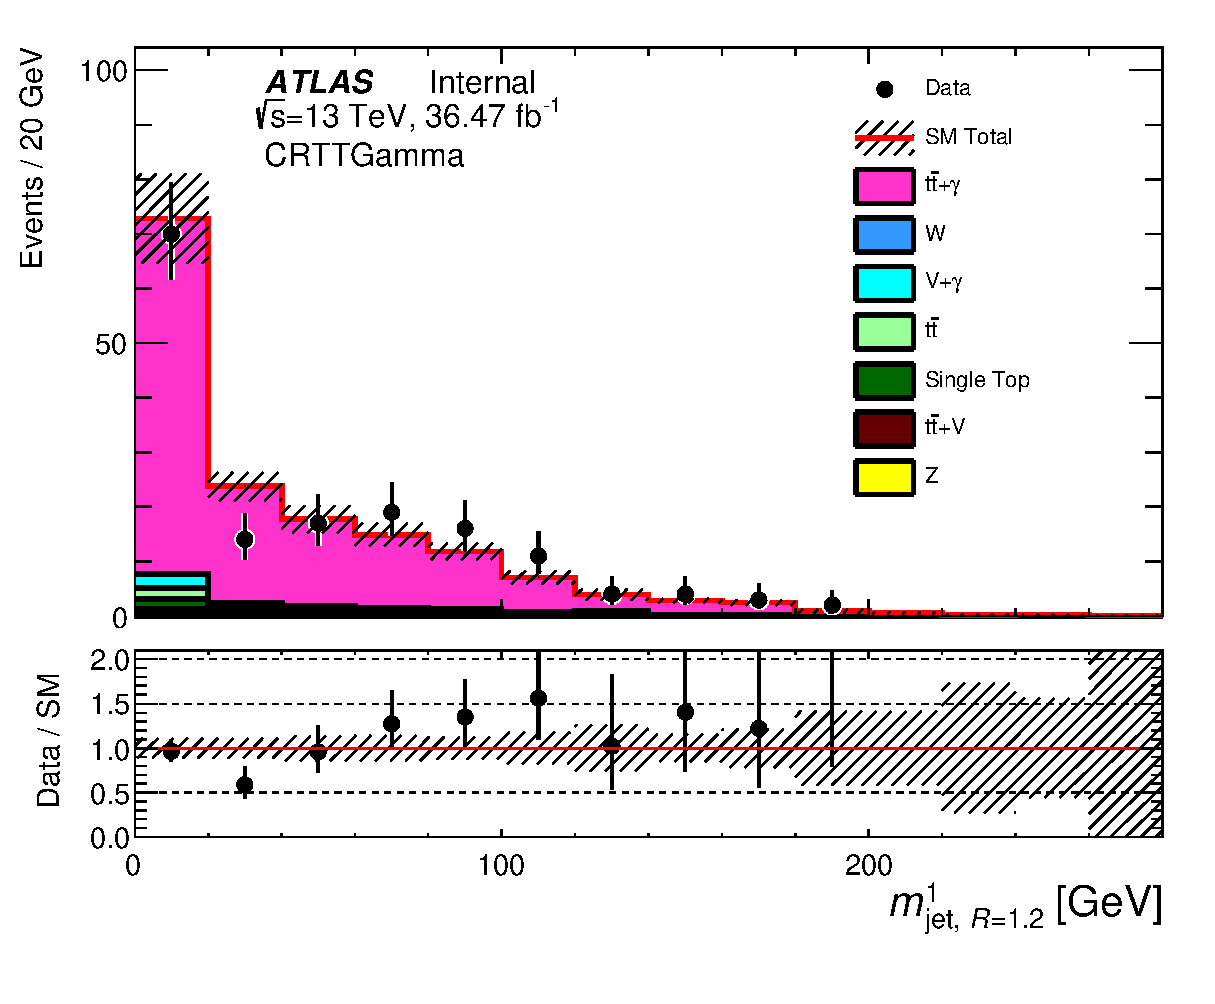
\includegraphics[width=0.49\textwidth]{figures/ttGamma/postfit/AntiKt12M_1__CRTTGamma.eps}
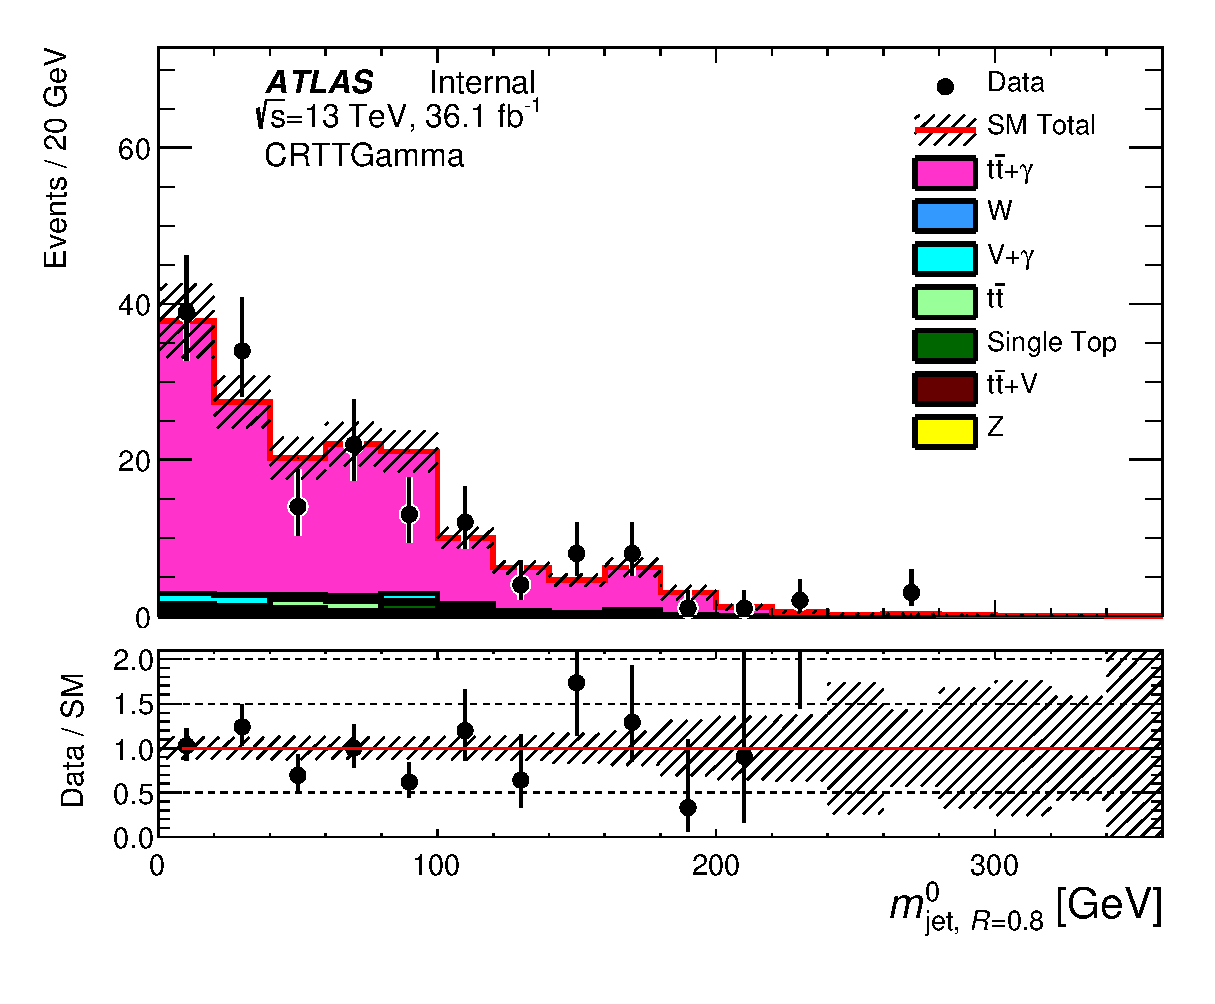
\includegraphics[width=0.49\textwidth]{figures/ttGamma/postfit/AntiKt8M_0__CRTTGamma.eps}
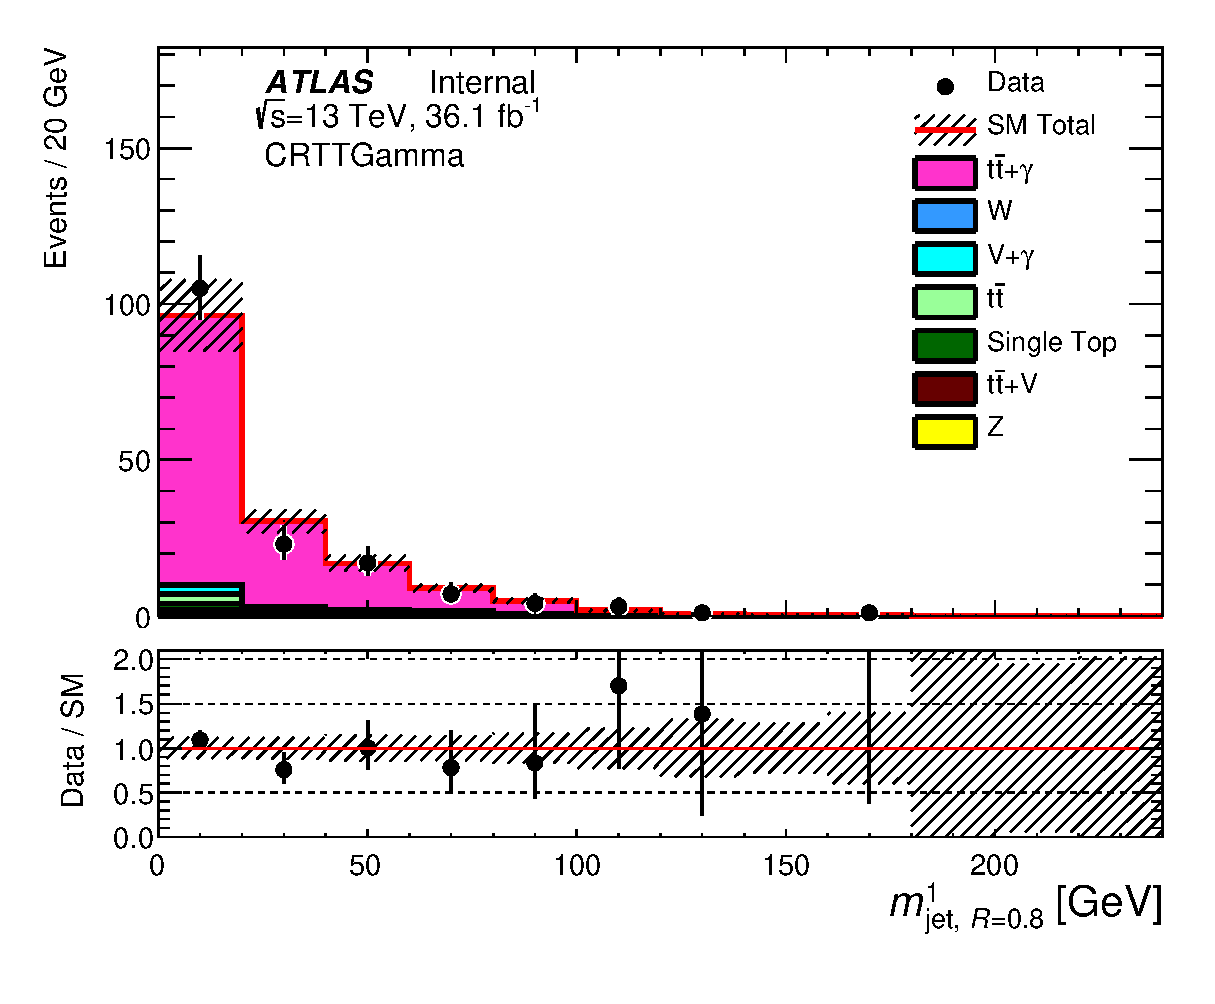
\includegraphics[width=0.49\textwidth]{figures/ttGamma/postfit/AntiKt8M_1__CRTTGamma.eps}
\caption{\label{fig:ttVMasses} Postfit distributions of the \pT\ of the
  leading and subleading jets for the 2 b-jets selection. The ratio between data and MC is given in the bottom panel. The hashed area in both the top and lower panel represents the uncertainty due to MC statistics.}
\end{center}
\end{figure}



Truth studies are performed in order to check the differencies in
kinematic distributions. The truth \pT\ ratio for a 2-bjet
selection are shown in Fig.~\ref{fig:ttZ_vs_ttGamma_pt}.

\begin{figure}[htpb]
\centering
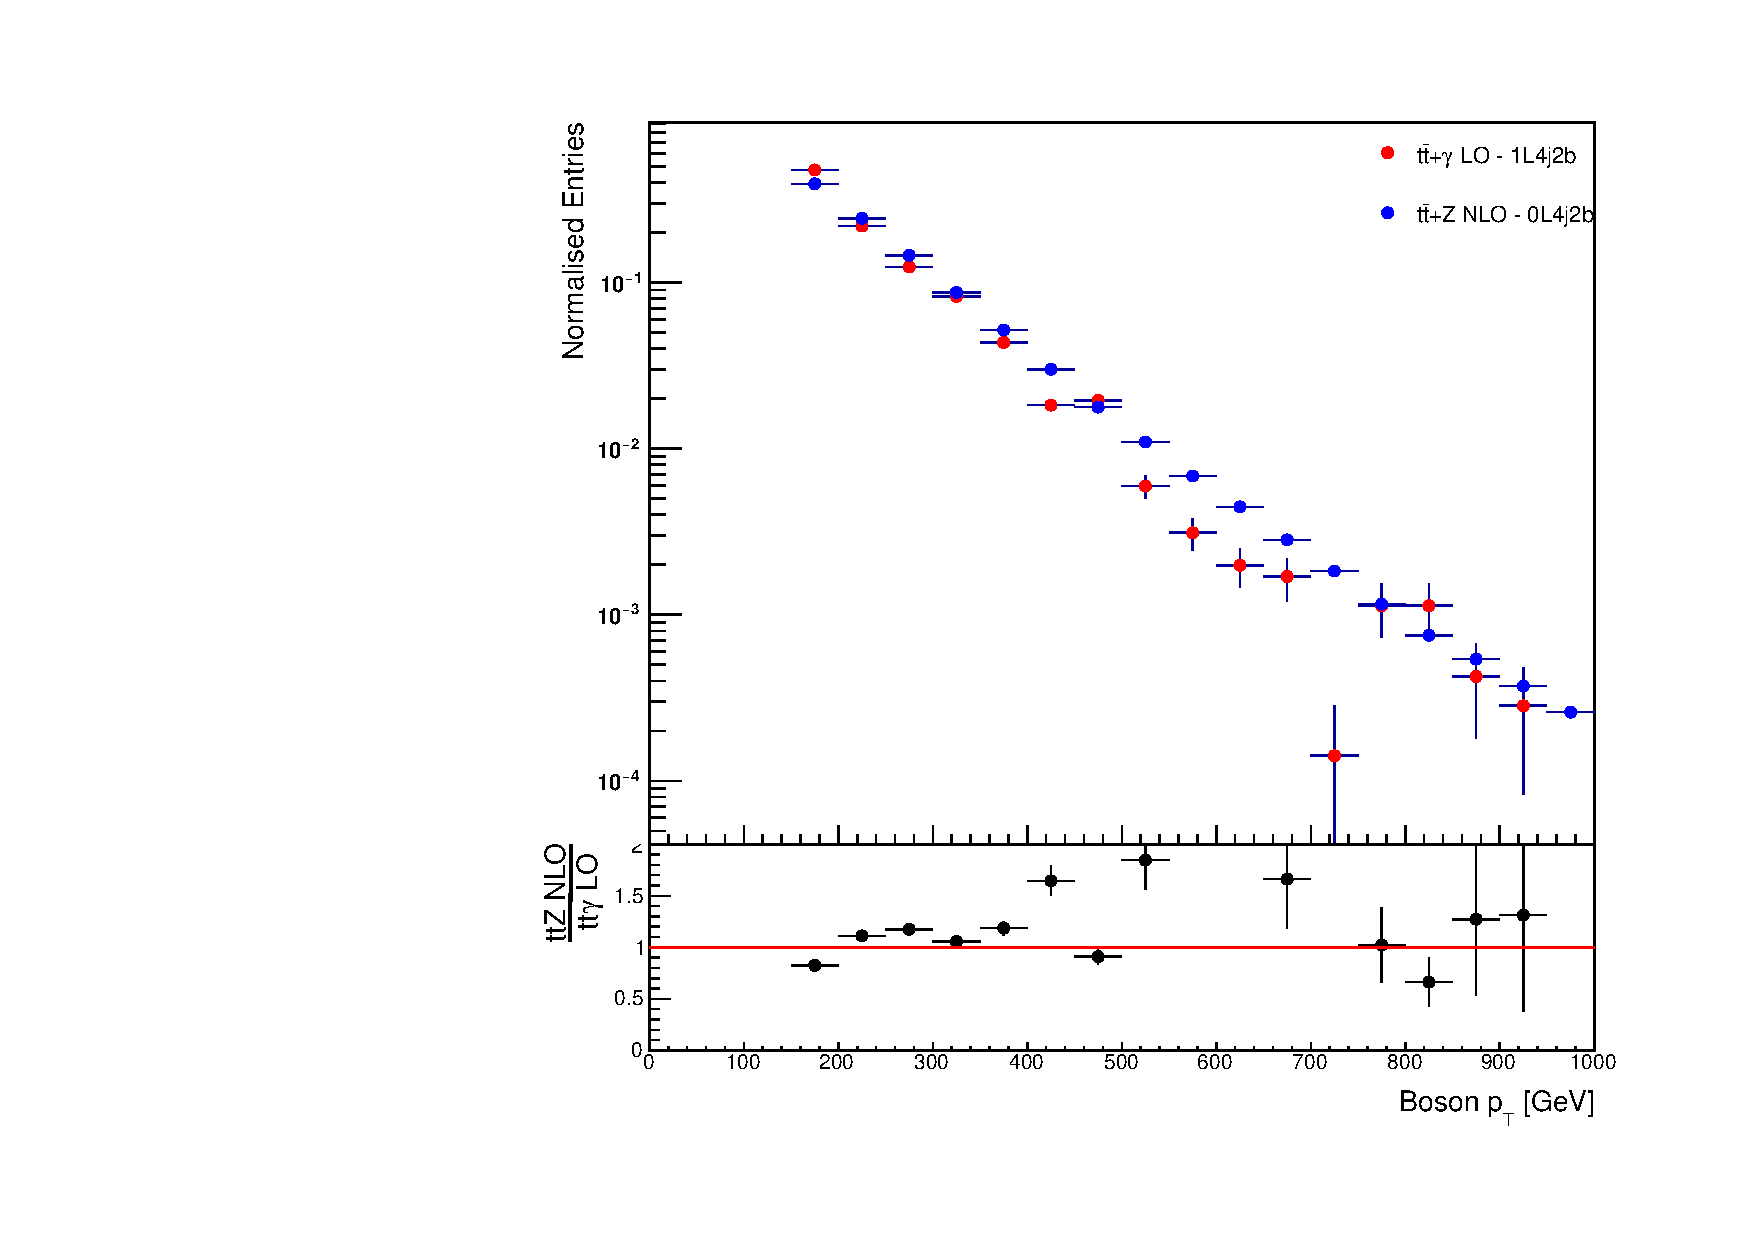
\includegraphics[scale=0.4]{figures/ttGamma/TruthStudies/Pt150}
\caption{Truth \pT\ ratio.}
\label{fig:ttZ_vs_ttGamma_pt}
\end{figure}






\clearpage

